\chapter{Experimental Setup}
Two open-source controllers operating systems were compared. Ryu and Pox are installed on a server machine. Conversely, Mininet and CBench are introduced on two distinctive host machines in the accompanying equipment and programming arrangements.

 \begin{table}[!hbt]
    \centering
    \caption{Features of Pox and Ryu \cite{ryuandpox}}
    \begin{tabular}{|p{4cm}|p{4cm}|p{4cm}|}
    \hline
         \textbf{Features} & \textbf{Pox} & \textbf{Ryu} \\ \hline
         Platform Support & Windows, Linux, Mac & Linux \\ \hline
    Last Updated & Nov 2017 & May 2020 \\ \hline
    License Provider & Apache & Apache \\ \hline
    Distributed Support & No & Yes \\ \hline
         Learning Curve & Easy & Moderate \\ \hline
         GUI & Yes & Yes \\ \hline
    REST API & Yes & Yes \\ \hline
    OpenFlow Version & v1.0 & v1.0 to v1.5, Niciria extensions \\ \hline
    \end{tabular}
    \label{RyuvsPox}
    \end{table}
    
\section{Hardware Configuration}
    \begin{table}[!hbt]
    \centering
    \caption{Physical constraints of Server and Host Machines}
    \begin{tabular}{|c|c|}
    \hline
    Architecture & x86\_64 \\ \hline
         CPU op-mode(s) & 32-bit, 64-bit \\ \hline
         CPU(s) & 8 \\ \hline
         Thread(s) per core & 2 \\ \hline
         Vendor ID & GenuineIntel \\ \hline
    Model name & Intel(R) Core(TM) i7-4790K CPU @ 4.00GHz \\ \hline
    L1d cache & 128 KiB \\ \hline
    L1i cache & 128 KiB \\ \hline
    L2 cache & 1 MiB \\ \hline
    L3 cache & 8 MiB \\ \hline
    \end{tabular}
    \label{Hardware}
    \end{table}

The setups, as referenced above, were not deliberately picked; rather, it was the asset limitations during the task's time. All things considered, these designs could be additionally changed dependent on rehashed tests. Thus, even the most exceedingly terrible performing controller is best considering the constrained processor and RAM.

\section{Software \& Tools}
The controller is run on a Linux Ubuntu Server 18.04 LTS OS so that it got dedicated RAM and processor cores \cite{resshare1970}, and 5 out of 8 cores were isolated for the controller using \textit{isolcpus} tool.

Perf was also installed along with the controllers on the server machine itself but on a different single isolated core to prevent influence from any other running process(s).

Oracle VM VirtualBox is installed on two separate host machines. An instance of Linux Ubuntu Desktop 16.04.02 LTS OS is created.

Mininet is installed on the Host OS and is for setting the switches, hosts, controllers, and for setting various possible connection combinations.

CBench device copies a lot of hosts per switch and switches and interfaces for SDN controller indicated. Generally, it creates them in the network and measures the presentation of the controller in 2 modes.
    \begin{itemize}
        \item Latency Mode: Packets in these events come in bulk from each switch.
        \item Throughput Mode: Packets in events come in sequential order.
    \end{itemize}

\begin{figure}[!hbt]
    \centering
        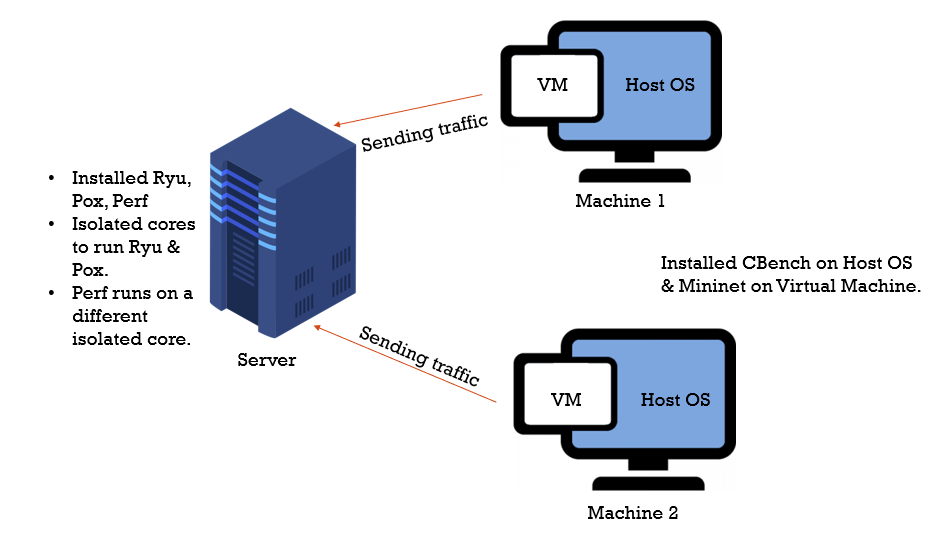
\includegraphics[width=\textwidth,keepaspectratio]{images/setup.png}
       \caption{Experimental Setup}
        \label{experimentalsetup}
\end{figure}

\begin{figure}[!hbt]
    \centering
        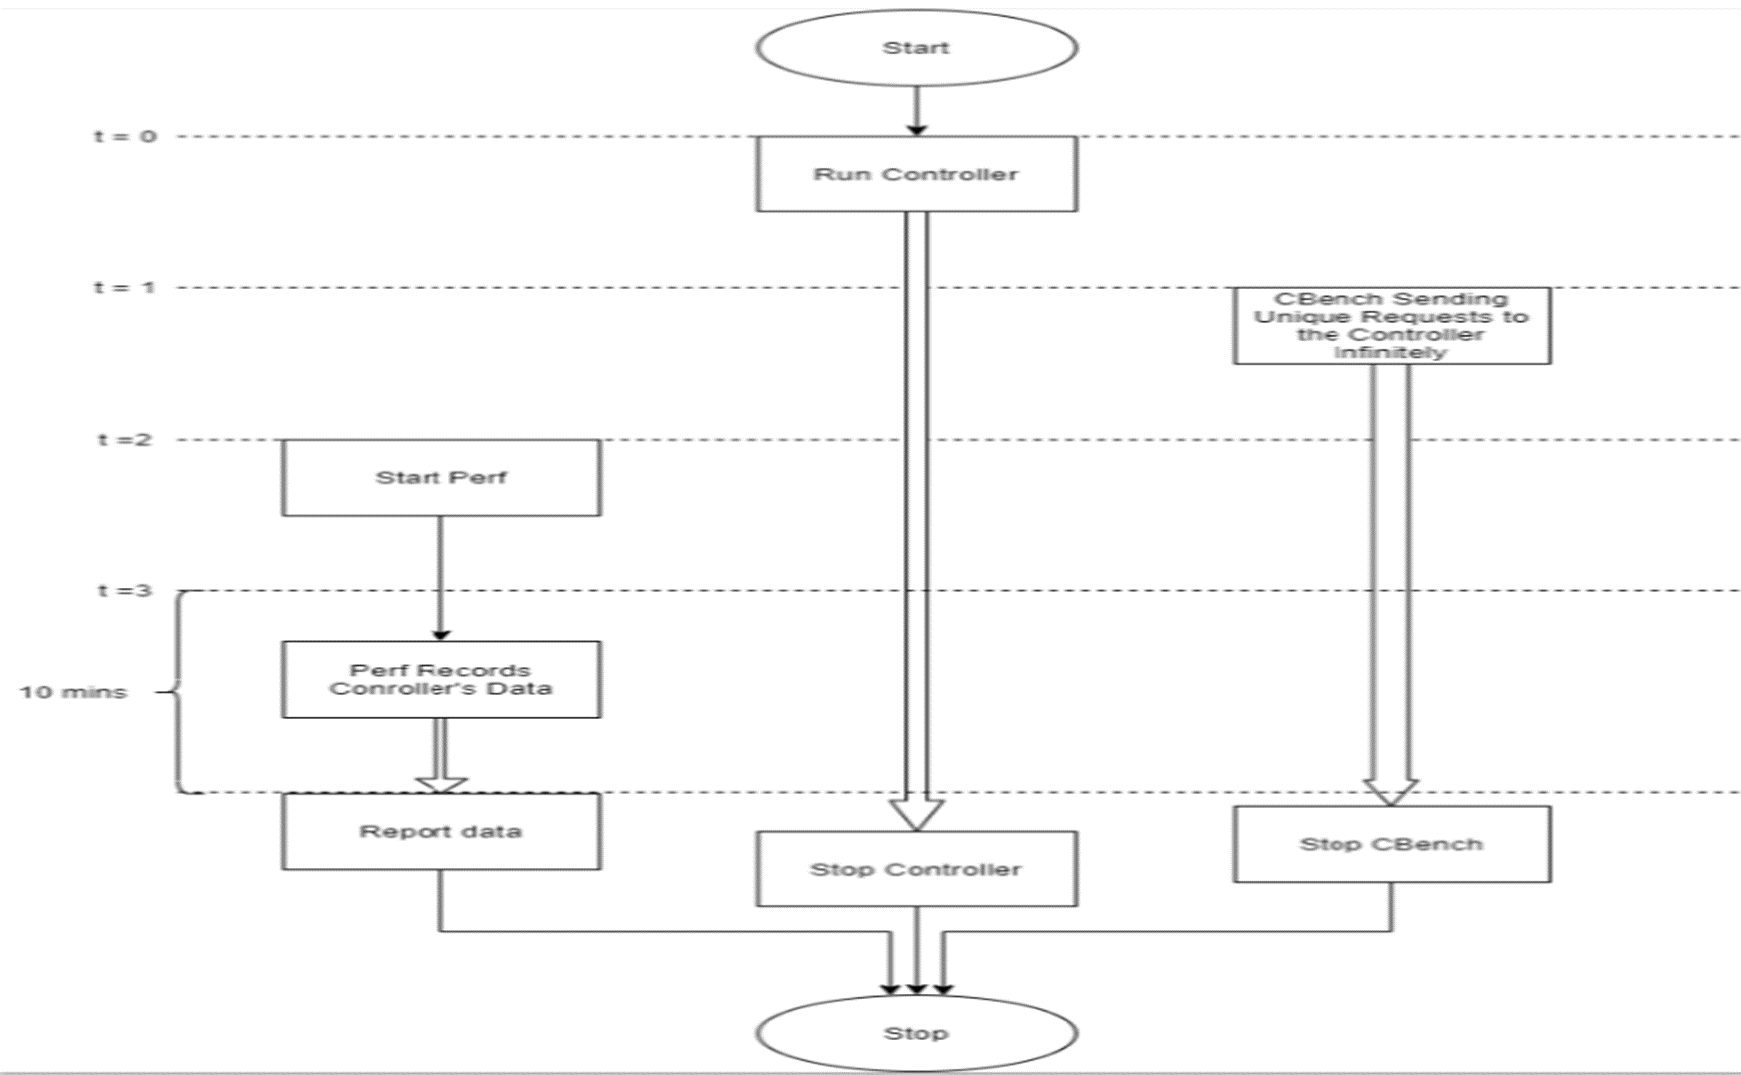
\includegraphics[width=\textwidth,keepaspectratio]{images/Workflow.PNG}
       \caption{Workflow of the Experiment}
        \label{workflowexperiment}
\end{figure}

However, in our case, we took the usage of CBench in throughput mode and generated massive traffic for the controller.

The overall experimental setup can be viewed as in Fig. \ref{experimentalsetup}. The Ryu and Pox along with perf, are installed on server machine, and whenever they are run, were run on isolated cores. In the experiment, 6 isolated cores are assigned for Pox. In one of the isolated core, perf is allowed to run. In the experiment, there are 2 hosts / client machines used. These two machines was set to send traffic to the server where controller is running. In both of the hosts, CBench is installed, and further Mininet is installed on a separate virtual machine in the system.

The experiment is carried on as the per the workflow, depicted in the Fig. \ref{workflowexperiment}. The controller is allowed run on isolated cores. Then the CBench and Mininet is allowed to send random packets to the running controller from other two remote machines. Perf tool is run to record the cores where controller is running for specified time and later stopped. This is done for both Ryu and Pox, and a number of times (here 5 times) to get relatively more accurate information. The information collected is further displayed in graphical chart using Google Chart.